% Vorlage für eine Bachelorarbeit
% Siehe auch LaTeX-Kurs von Mathematik-Online
% www.mathematik-online.org/kurse
% Anpassungen für die Fakultät für Mathematik
% am KIT durch Klaus Spitzmüller und Roland Schnaubelt Dezember 2011

\documentclass[12pt,a4paper]{scrartcl}
% scrartcl ist eine abgeleitete Artikel-Klasse im Koma-Skript
% zur Kontrolle des Umbruchs Klassenoption draft verwenden


% die folgenden Packete erlauben den Gebrauch von Umlauten und ß
% in der Latex Datei
\usepackage[utf8]{inputenc}

%\usepackage[latin1]{inputenc} %  Alternativ unter Windows
\usepackage[T1]{fontenc}
%\usepackage[ngerman]{babel}
%\usepackage{parskip}

%\usepackage{nicefrac}


\usepackage[pdftex]{graphicx}
\usepackage{latexsym}
\usepackage{amsmath,amssymb,amsthm}
\usepackage[disable]{todonotes}

\usepackage{tikz}
%\usetikzlibrary{automata,positioning}

% Abstand obere Blattkante zur Kopfzeile ist 2.54cm - 15mm
\setlength{\topmargin}{-15mm}

%\setlength{\parindent}{0pt}


% Umgebungen für Definitionen, Sätze, usw.
% Es werden Sätze, Definitionen etc innerhalb einer Section mit
% 1.1, 1.2 etc durchnummeriert, ebenso die Gleichungen mit (1.1), (1.2) ..
\theoremstyle{plain}
\newtheorem{Theorem}{Theorem}[section]
\newtheorem{Lemma}[Theorem]{Lemma}	
\newtheorem{Remark}[Theorem]{Remark} 

\theoremstyle{definition}
\newtheorem{Definition}[Theorem]{Definition} 
\newtheorem{Example}[Theorem]{Example}
	   
                  
\numberwithin{equation}{section} 

% einige Abkuerzungen
\newcommand{\C}{\mathbb{C}} % komplexe
\newcommand{\K}{\mathbb{K}} % komplexe
\newcommand{\R}{\mathbb{R}} % reelle
\newcommand{\Q}{\mathbb{Q}} % rationale
\newcommand{\Z}{\mathbb{Z}} % ganze
\newcommand{\N}{\mathbb{N}} % natuerliche
\newcommand{\2}{\mathbb{Z} / 2 \mathbb{Z}}
\newcommand{\G}{\mathcal{G}}
\newcommand{\1}{\bar{1}}
\newcommand{\0}{\bar{0}}
\newcommand{\widthrect}{160}
\newcommand{\widthrectb}{160}
\newcommand{\heightrect}{4}
\newcommand{\abstrect}{10}


\renewcommand{\labelenumi}{\roman{enumi})}



\begin{document}
  % Keine Seitenzahlen im Vorspann
  \pagestyle{empty}

  % Titelblatt der Arbeit
  \begin{titlepage}

    
\includegraphics[scale=0.45]{kit-logo.jpg} 
    \vspace*{2cm} 

 \begin{center} \large 
    
    Masterarbeit
    \vspace*{2cm}

    {\huge Turing machines and irrational values of $\ell^2$-Betti numbers}
    \vspace*{2.5cm}

    Jan Kohlmüller
    \vspace*{1.5cm}

    20.08.2017
    \vspace*{4cm}


    Betreuung: Roman Sauer \\[1cm]
    Fakultät für Mathematik \\[1cm]
		Karlsruher Institut für Technologie
  \end{center}
\end{titlepage}



  % Inhaltsverzeichnis
  \tableofcontents

\newpage
 


  % Ab sofort Seitenzahlen in der Kopfzeile anzeigen
  \pagestyle{headings}

\section{Introduction}


\section{$\ell^2$-Betti numbers}
At first we will give a short introduction into the theory of $\ell^2$-Betti numbers. For a wider approach see \cite{LUECK}. We will assume some basic knowledge about cellular homology and the associated Betti numbers. For more information on this topic see e.g. \cite{HATCH}. As an alternative a reader not familiar with these topics may just accept the results of \ref{MCW} and study the definitions given in section \ref{fiss}.

In this whole chapter $G$ is always a discrete countable group with multiplication $\cdot_G$.
\subsection{Von Neumann Dimension} \label{fiss}
At first let us begin with some basic definitions.
\begin{Definition} \label{GR}
	The \emph{group ring} $RG$ over a Ring $R$ is the free module over $G$ with the additional multiplication
	\begin{align*}
		\sum_{h \in H} \alpha_h \cdot h \cdot_{RG} \sum_{k \in K} \beta_k \cdot k = \sum_{h \in H} \sum_{k \in K} \alpha_h \beta_k \cdot h \cdot_G k
	\end{align*}
	with $\alpha_h, \beta_k \in R$ and $H, K \in G$ finite subsets.
\end{Definition}
If $R$ is a field then $RG$ is an algebra and in particular a vector space with dimension $|G|$ if $G$ is finite. We will often see the group ring $\C G$. If $G$ is infinite then $\C G$ is an infinite dimensional vector space with scalar product. In this case $\C G$ is not a Hilbert space. Therefore we will introduce the space $\ell^2(G)$ which is in fact the Hilbert space completion of $\C G$.
\begin{Definition}
	$\ell^2(G)$ is the Hilbert space consisting of formal sums $\sum_{g \in G} \lambda_g \cdot g$ such that $\lambda_g \in \C$ and $\sum_{g \in G} |\lambda_g|^2 < \infty$. The multiplication is defined as in \ref{GR} and the scalar product is defined through
	\begin{align*}
		\langle \sum_{g \in G} \alpha_g \cdot g, \sum_{g \in G} \beta_g \cdot g \rangle := \sum_{g \in G} \alpha_g \overline{\beta_g}.
	\end{align*}
\end{Definition}
\begin{Remark}
	If $G$ is a set instead of a group we can also define a Hilbert space $\ell^2(G)$. Of course we do not have a multiplication in this case.
\end{Remark}
We now want to define a dimension for spaces embedded in $\ell^2(G)$. In most cases the normal vector space dimension of these spaces will be infinite and therefore not useful. We will instead use the von Neumann dimension which requires some preliminary work.
\begin{Definition}
	The \emph{group von Neumann} algebra $\mathcal{N}(G)$ is defined as the algebra of $G$-equivariant bounded operators from $\ell^2(G)$ to $\ell^2(G)$ where $G$ acts on $\ell^2(G)$ by left multiplication.
\end{Definition}
We will denote the bounded operators of a Hilbert space $H_1$ with $\mathcal{B}(H_1)$. If $G$ acts on a Hilbert Space $H_2$ we will call the subspace of $G$-equivariant elements of $H_2$ by $H_2^G$. Therefore we can also define the group von Neumann algebra through $\mathcal{N}(G) := \mathcal{B}(\ell^2(G))^G$.
\begin{Definition}
	Let $e_G \in G$ be the unit element of $G$. Then
	\begin{align*}
		tr_{\mathcal{N}(G)}: \mathcal{N}(G) \to \C, A  \mapsto \langle A(1 \cdot e_G), 1 \cdot e_G \rangle
	\end{align*}
	is called the \emph{von Neumann trace} on $\mathcal{N}(G)$.
\end{Definition}
\begin{Remark}
	Right multiplication with an element of the group ring $\C G$ is a $G$-equivariant operator on $\ell^2(G)$ and therefore has a well defined von Neumann trace.
\end{Remark}
\begin{Definition}
	A \emph{Hilbert $\mathcal{N}(G)$-module} is a Hilbert space $H$ with a linear isometric $G$-action such that there exists an isometric linear $G$-embedding from $H$ to $\ell^2(G)^n$ for some $n \in \N$.
\end{Definition}
\begin{Definition}
	Let $H$ be a Hilbert $\mathcal{N}(G)$-module with corresponding embedding \\ $\iota: H \to \ell^2(G)^n$ and let $pr_{\iota(H)}: \ell^2(G)^n \to H$ be the corresponding $G$-equivariant projection. Let $\iota_i: \ell^2(G) \to \ell^2(G)^n, y \mapsto (x_1, \ldots, x_n)$ with $x_j = \delta_{i,j} \cdot y$ be the inclusion of the i-th $\ell^2(G)$ and $pr_i: \ell^2(G)^n \to \ell^2(G), (x_1, \ldots, x_n) \mapsto x_i$ the corresponding projection. Then 
	\begin{align*}
		tr_{\mathcal{N}(G)}: \mathcal{B}(H)^G \to \C, A \mapsto \sum_{i = 1}^{n} tr_{\mathcal{N}(G)}(pr_i \circ \iota \circ A \circ pr_{\iota(H)} \circ \iota_i)
	\end{align*}
	is called the \emph{von Neumann trace} on $H$.
\end{Definition}
One can show that the trace is independent of the chosen embedding and therefore well-defined.
\begin{Definition}
	Let $H$ be a Hilbert $\mathcal{N}(G)$-module. We define the \emph{von Neumann dimension} of $H$ as
	\begin{align*}
		dim_{\mathcal{N}(G)}(H) = tr_{\mathcal{N}(G)}(id_H).
	\end{align*}
\end{Definition}
\begin{Remark}
	Let $H \subset \ell^2(G)$ be a $G$-equivariant subset and $pr_H: \ell^2(G) \to H$ a $G$-equivariant projection. Then\begin{align*}
	dim_{\mathcal{N}(G)}(H) = tr_{\mathcal{N}(G)}(pr_H) = \langle pr_H (1 \cdot e_G), 1 \cdot e_G \rangle.
	\end{align*}
\end{Remark}
\todo{ueberall g-equivariant ueberpruefen}

\subsection{$\ell^2$-Betti numbers of $G$-CW-complexes}
One can now define the $\ell^2$-Betti numbers of CW-complexes in a very similar way as for cellular homology. But first we have to define a group action on CW-complexes.
\begin{Definition}
	Let $X$ be a CW-complex and $\rho: G \to Homeo(X)$ an action of $G$ on $X$ by homeomorphism such that for every open cell $E \subset X$ and every $g \in G$ it holds that $\rho(g)(E)$ is again an open cell and $\rho(g)|_{E} = id_E$ if $\rho(g)(E) \cap E \neq \emptyset$. Then $\rho$ is called a \emph{cellular action}.
\end{Definition}

\begin{Definition}
	A \emph{$G$-CW-complex} is a CW-complex together with a cellular $G$-action.
\end{Definition}

\begin{Definition}
	The \emph{orbit} of an $n$-cell in a $G$-CW-complex is called a $G$-equivariant $n$-cell.
\end{Definition}

\begin{Definition}
	Let $X$ be a $G$-CW complex. $X$ is called
	\begin{itemize}
		\item \emph{proper} if all stabilizer groups are finite,
		\item \emph{free} if all stabilizer groups are trivial,
		\item \emph{finite type} if for every $n \in \N$ it has only finitely many $G$-equivariant $n$-cells.
	\end{itemize}
\end{Definition}

\begin{Remark}
	One can show that the chain complex of a $G$-CW complex $X$ is a chain complex $C_*(X)$ of left $\Z G$-modules, i.e. each $C_n(X)$ is a left $\Z G$-module and the differentials are homomorphisms of these modules.
\end{Remark}
\begin{Definition}
	The \emph{$\ell^2$-chain complex} of a $G$-CW complex $X$ is
	\begin{align*}
		C_*^{(2)}(X) = \ell^2(G) \otimes_{\Z G} C_*(X).
	\end{align*}
\end{Definition}

\begin{Definition}
	Let $X$ be a proper, finite type $G$-CW complex and $C_*^{(2)}(X)$ the corresponding $\ell^2$-chain complex with its differential $d_*^{(2)}$. Then 
	\begin{align*}
		H_n^{(2)}(X) := \ker(d_n^{(2)}) / \overline{im(d_{n+1}^{(2)})}
	\end{align*}
	is called the \emph{$n$-th $\ell^2$-homology} and 
	\begin{align*}
		b_n^{(2)}(X)=dim_{\mathcal{N}(G)}H_n^{(2)}(X)
	\end{align*}
	the \emph{$n$-th $\ell^2$-Betti number}.
\end{Definition}
\begin{Remark}
	One can show that for a proper, finite type $G$-CW complex $H_n^{(2)}(X)$ is a Hilbert $\mathcal{N}(G)$-module and therefore the $\ell^2$-Betti number is in fact well-defined.
\end{Remark}

\subsection{$\ell^2$-Betti numbers arising from a group}
We will now show that it is sufficient for our purpose to calculate the von Neumann trace of the kernel of elements of the group ring without mentioning CW-complexes.
\begin{Remark}\label{MAB}
	A matrix $A \in \C G^{n \times m}$ can be seen as a map from $\ell^2(G)^n \to \ell^2(G)^m$ via $x \mapsto x^{\top} \cdot A$. We will refer to this map also by $A$. Be aware that if $G$ is not abelian this is not the same map as $A^\top x$.
\end{Remark}
\begin{Lemma}
	For a matrix $A \in \C G^{n \times m}$ $\ker(A)$ is a Hilbert $\mathcal{N}(G)$-module and therefore has a well-defined von Neumann-dimension.
\end{Lemma}
\begin{proof}
	Of course $\ker(A)$ is a subspace of $\ell^2 (G)^n$. We can use $id|_{\ker(A)}$ as embedding. It remains to show that $\ker(A)$ is closed under the natural $G$-action on $\ell^2 (G)^n$. So let $x \in \ker(A)$ be an element in the kernel and $g \in G$ be an element of the group. It now holds that
	\begin{align*}
		(g \cdot x)^\top \cdot A = g \cdot (x^\top A) = g \cdot 0 = 0
	\end{align*}
	because the action is linear.
\end{proof}
\begin{Theorem} \label{MCW}
	Let $x \in \R$ and $G$ be a discrete, countable, finitely generated group. The following are equivalent:
	\begin{enumerate}
		\item There exists a cocompact free finite type $G$-CW-complex $X$ and an integer $n \in \N$ such that $b_n^{(2)}(X)=x$.
		\item There exists a matrix $A \in \Q G^{n \times n}$ for an integer $n \in \N$ such that \newline $dim_{\mathcal{N}(G)}(\ker (A))=x$.
	\end{enumerate}
\end{Theorem}
\begin{proof}
	$"i) \Rightarrow ii)"$ Let $X$ be a cocompact free finite type $G$-CW-complex and $n \in \N$ such that $b_n^{(2)}(X)=x$. We define 
	\begin{align*}
		\Delta_n^{(2)} = d_n^{(2)*} d_n^{(2)} + d_{n+1}^{(2)} d_{n+1}^{(2)*},
	\end{align*}
	which is a map from $C_n^{(2)}(X)$ to $C_n^{(2)}(X)$. The differential can be written as a matrix $A' \in \Z G$ and therefore $\Delta_n^{(2)}$ also lies in $\Z G$. It remains to show that $\ker(\Delta_n^{(2)}) = H_n^{(2)}$ holds. 
	
	$"ii) \Rightarrow i)"$ Let $n \in \N$ and $A\in \Q G^{n \times n}$. Because $k \cdot A$ has the same kernel as $A$ for every $k \in \Z$ we can assume that $A \in \Z G^{n \times n}$. The corresponding map will be also called $A$. We will construct a $G$-CW-complex $X$ with $d_3^{(2)} = A$ and $d_4^{(2)}$ trivial. Therefore $H_3^{(2)}(X) = \ker(A)$ and $i)$ follows.
	
	First we can see that a graph can always be seen as a CW-complex with the edges as 1-cells and the vertices as 0-cells. Let $g_1 \ldots g_m$ be generators of $G$ and let $Y$ be the corresponding Cayley graph of $G$ which has a natural cellular free $G$-action and is therefore a free, finite type $G$-CW-complex. In addition it has exactly $1$ $G$-equivariant $0$-cell and $m$ $G$-equivariant $1$-cells and no other cells. We then glue $n$ many $2$-cells on each $0$-cell, i.e. we attach them via the attaching map which sends all of $S^1$ to a single point. 
	
	We now glue in $n$ many $G$-equivariant $3$-cells in such a way that $A$ corresponds to $d_3^{(2)}$:
	Let $A_{ij} = \sum_{g \in G} z_{(g, i, j)} g \in \Z G$ denote the entry in the i-th row and the j-th column of $A$. We fix one $0$-cell and call it $e$ and we call the corresponding $2$-cells $e_1 \ldots e_n$. We glue in $G \times D^3$ where each element $h \times D^3$ is glued $z_{(g, 1, j)}$ many times to $h g \cdot e_j$ for each $g \in G$ and $j \in \{1, \ldots, n\}$. We then see that $d_3^{(2)}$ maps the vector $(\sum_{g \in G} \lambda_g g, 0 , \ldots , 0) \in (\ell^2 G)^n$ to $(\sum_{g \in G} \sum_{h \in H} \lambda_g z_{(h, 1, 1)} g h, \ldots , \sum_{g \in G} \sum_{h \in H} \lambda_g z_{(h, 1, n)}) \in (\ell^2 G)^n$. We then repeat this for every row of $A$ and get that $d_3^{(2)} = A$. The resulting $G$-CW-complex $X$ is still free, finite type and because $X/G$ is finite $X$ is cocompact.
\end{proof}
\todo{\ker(delta) = homology zeigen? Graphik und etwas genauer?}
\begin{Remark}
	One can show that \ref{MCW} also holds if $G$ is not finitely generated.
\end{Remark}
\begin{Definition}
	We say that a number $x \in \R$ \emph{arises} from a discrete countable group $G$ if it fulfills one (and therefore both) of the conditions of \ref{MCW}.
\end{Definition}
The statement of \ref{MCW} will be implicitly used in many points of this work. In fact we will never construct a $G$-Cw-complex and instead construct an element of a group ring $\Q (G)$ of $G$ which kernel has the desired von Neumann dimension.


\begin{Lemma}\label{add}
	If $x \in \R$ and $z \in \R$ both arise from a discrete, countable group $G$, then so does $x + z$.
\end{Lemma}
\begin{Lemma}\label{mult}
	Let $G$ is a discrete countable group and $H$ a discrete finite group. If $x \in \R$ arises from $G \times H$ then $x \cdot |H|$ arises from $G$.
\end{Lemma}
\todo{Vllt. noch beweisen oder Quelle}
\section{Turing dynamical systems}
To fix notation we will first give a definition of a Turing machine. For convenience we will only allow 1 and 0 as symbols on our tape.
\begin{Definition}
	A \emph{Turing machine} is a 5-tuple $T=(S,\delta, A, R, I)$ where S is a finite set of states and 
	\begin{align*}
		\delta: \2 \times S \setminus(A \cup R) \to \2 \times \{-1, 0, 1\} \times S
	\end{align*}
	is called the transition function. $A \subset S$ is called the set of accepting states, $R \subset S$ is called the set of rejecting states and $I \in S$ is called the initial state.
	A Turing machine is \emph{read-only} if $\delta$ fixes the $\2$-coordinate, i.e.
	\begin{align*}
		\delta (x, \sigma) = (x, \beta, \tilde{\sigma})
	\end{align*}
	for each $x \in \2$ and $\sigma \in S \setminus(A \cup R)$.
\end{Definition}
In addition each Turing machine uses a "tape", i.e. a set $\Z / 2\Z ^{\Z}$ with a "head" on the element corresponding to the index 0. A Turing machine can operate on an element of $Y \in \Z / 2\Z ^{\Z}$ which is called an input. We start with the initial state and use the transition function $\delta$ to get $\delta(Y_0, I)$. The first coordinate corresponds to the new element $Y_0$, the third to the new state and the second corresponds to shifting the tape to the left or the right and therefore getting a new $Y_0$, e.g. if $\delta(I, Y_0)_3 = 1$ we shift the whole tape one to the left, therefore our new $Y_0$ is our old $Y_1$. We repeat this step until we get a state in $A \cup R$. We say that the Turing machine accepts $Y$ if we get a state in $A$ after finitely many steps and it rejects $Y$ if we get a state in $R$ after finitely many steps. We say that the Turing machine holds for $Y$ if it accepts or rejects it.

For the purpose of calculating $\ell^2$-Betti numbers of groups we need to extend this definition. Let $(X, \mu)$ be a probability measure space divided into finitely many disjoint measurable subsets $X_i$. Let $\Gamma$ be a countable discrete group and $\rho$ be a right measure preserving action of $\Gamma$ on X.
We now choose 3 disjoint subsets $A$, $R$, $I$, where each of them is a union of certain $X_i$. They will be called the accepting set, the rejecting set and the initial set. In addition we choose a $\gamma_i \in \Gamma$ for each $X_i \subset X$ such that for each $i$ with $X_i \subset A$ or $X_i \subset R$ it holds that $\gamma_i = e$ where $e$ is the neutral element in $\Gamma$. 
Let $Ind: X \to \N$ be the map which assigns to each $x \in X$ the corresponding index of the $X_i$ it is contained in.
\begin{Definition}
	 The map 
	 \begin{align*}
	 T_X:X \to X, x \mapsto \rho(\gamma_{Ind(x)})(x)
	 \end{align*}
	 is called the \emph{Turing map}.
	 The group $\Gamma$ and the space $X$ (with all the choices of subsets and corresponding $\gamma_i$ made in the last paragraph) together with the Turing map will be called a \emph{Turing dynamical system} and will be denoted by $(T_X)$
\end{Definition}
Let $x \in X$ be an element of $X$. If there is a $k \in \N$ such that $T_X^k(x) = T_X^{k + 1}(x)$ there also holds $T_X^h(x) = T_X^{h + 1}(x)$ for all $h \in \N$ with $h \geq k$. We then define $T_X^\infty (x) = T_X^k(x)$. Mostly we don't look at the map $T_X$ but the map $T_X^\infty$. We say that the Turing dynamical system $(T_X)$ accepts an input $y \in I$ if $T_X^\infty(y) \in A$ and it rejects it if $T_X^\infty(y) \in R$. In addition we say that $(T_X)$ holds for $y$ if it accepts or rejects it.

For every Turing machine $T$ we can construct a Turing dynamical system $(T_X)$ which does the same as the Turing machine, i.e. we have a bijection $\Psi: \2^\Z \to I$ such that $T$ accepts (rejects) an input $Y \in \2^\Z$ if and only if $(T_X)$ accepts (rejects) $\Psi(Y)$. This allows us to first define a Turing machine and the get a Turing dynamical system out of it. We will use this fact may times in chapter \ref{chlamplighter}. The following example shows how the corresponding Turing dynamical system is constructed. But first let us fix notation.
\begin{Remark}
	Let $M \subset N^\Z$  be defined through 
	\begin{align*}
		M = \{(n_i)_{i \in \Z} \in N^\Z | n_{-k} = m_{-k}, \cdots, n_l = m_l \} \ k,l \in \N,
	\end{align*}
	i.e. a set where $k+l$ coordinates including the $0$-coordinate are fixed. We then simply write $[m_{-k} \cdots \underline{m_0} \cdots m_l]$ for $M$ and $[m_{-k} \cdots \underline{m_0} \cdots m_l][\sigma]$ for $M \times \{\sigma\}$.
\end{Remark}
\begin{Example}\label{TMtoTDS}
	Let  $T=(S,\delta, \tilde{A}, \tilde{R}, \tilde{I})$ be a Turing machine. We define $X = \2^\Z \times S$ and $\Gamma =   \2 \times \Z \times Bij(S)$.
	The action of $\Gamma$ on $X$ is defined by the following rules:
	\begin{itemize}
		\item The generator $\1$ of the group $\Z / 2\Z$ acts on the $\Z / 2\Z^\Z$ part of $X$ by adding $\1$ to the element with index $0$.
		\item The generator $1$ of the group $\Z$ acts also on the $\Z / 2\Z^\Z$ part by shifting every element 1 to the left, i.e. decreasing the index of every element by 1.
		\item $Bij(S)$ acts on $S$ in the natural way.
	\end{itemize}
	We will now use the transition function to construct the Turing map. We choose the following devision of $X$:
	\begin{align*}
	X = \bigcup_{x \in \2, \sigma \in S} [\underline{x}][\sigma].
	\end{align*}
	For an arbitrary $X_i = [\underline{x}][\sigma]$ we can use the transition function of the Turing machine. Let
	\begin{align*}
		(\alpha, \beta,\tilde{\sigma}) = \delta(x, \sigma)
	\end{align*} 
	denote  the image of $(x, \sigma)$. \\
	Now let $\tau \in Bij(S)$ be some map which sends $\sigma$ to $\tilde{\sigma}$ and let $y \in \2$ be $y=x-\alpha$. We can then see $y$ as a map from $\2$ to itself which sends $x$ to $\alpha$. Our element $\gamma_i$ corresponding to $X_i$ is then given by 
	\begin{align*}
		\gamma_i = \begin{cases}
			(\0, 0, id) & if \ X_i \subset A \cup R \\
			(y, \beta, \tau) & otherwise
		\end{cases}.
	\end{align*} 
	We only need to define $A$, $R$ and $I$. $A$ is given by
	\begin{align*}
	A = \bigcup_{x \in \2, \sigma \in \tilde{A}}[\underline{x}][\sigma]
	\end{align*}
	which is of course a union of some $X_i$. $R$ and $I$ can be defined analogous. 
	
	The resulting Turing dynamical system $(T_X)$ accepts (rejects) an element in the initial set $Y \times \tilde{I} \subset I$ exactly when the Turing machine $T$ accepts (rejects) the input $Y \in \2^\Z$.
\end{Example} 
Our ultimate goal is to use Turing dynamical systems to get $\ell^2$-Betti numbers arising from a group. For this purpose some additional definitions and restrictions are needed.
\begin{Definition}
	The \emph{first fundamental set} $\mathcal{F}_1(T_X)$ is the subset of $I$ consisting of those points $x$ with $T_X^\infty(x) \in A$ and there is no point $y$ with $T_X(y)=x$. The \emph{second fundamental set} is the subset of $A$ defined as $\mathcal{F}_2(T_X)=T_X^\infty(\mathcal{F}_1(T_X))$. The \emph{first (second) fundamental value} $\Omega_1(T_X) \ ( \Omega_2(T_X))$ is the measure of the corresponding fundamental set.
\end{Definition}

\begin{Definition}
	We say that a Turing dynamical system $(T_X)$
	\begin{itemize}
		\item \emph{stops at any configuration} if $T_X^\infty (x) \in A \cup R$ for almost all $x \in X$,
		\item \emph{has disjoint accepting chains} if $T_X^\infty (x) \neq T_X^\infty (y)$ for almost all $x, y \in \mathcal{F}_1(T_X)$ with $x \neq y$,
		\item \emph{does not restart} if the set $T_X(X) \cap I$ has measure $0$.
	\end{itemize}
\end{Definition}
 

\begin{Definition}
	Let $(T_X)$ be a Turing dynamical system where $X = \Pi_{j \in J} \2$ is an infinite product of $\2$ equipped with the normalized Haar measure and each $X_i$  has only finitely many fixed elements, i.e. is of the form $X_i = \{(x_j)_{j \in J} \in X \ | \ x_k = \0 \ \forall k \in I_1, x_h = \1 \ \forall h \in I_2\, \ I_1, I_2 \subset J \ \text{finite}\}$. If in addition the action of $\Gamma$ is by continuous group automorphisms and $(T_X)$ stops at any configuration, has disjoint accepting chains and does not restart it is called a \emph{computing} Turing dynamical system.
\end{Definition}
\begin{Remark}
	For more information about Haar measure see e.g. \todo{Quelle fuer Haar measure}. For us it is only relevant that there always exists a unique normalized left Haar measure on $G$ if $G$ is a locally compact Hausdorff topological group. In addition the Haar measure is left translation invariant.
\end{Remark}
 
Before we give an example of a computing Turing dynamical system we fix the notation of the shifting operation, because we will need it later on.
\begin{Definition} \label{shift}
	An element $z \in \Z$ acts on $\2^{\Z} = \prod_{i \in \Z} \2$ by decreasing every index by $z$. We call this action the shift action and denote it by $\zeta$. $\Z$ acts on $\bigoplus_{i \in \Z} \2$ in the same way which we will also call $\zeta$.
\end{Definition}
Of course the Turing dynamical system constructed in \ref{TMtoTDS} is not computing in most cases. But for many read-only Turing machines a computing Turing dynamical system can be constructed in a similar way. In fact we will only use read-only Turing machines.
\begin{Example} \label{roTMtoTDS}
	Let $T$ be a read-only Turing machine. Let $(T_X)$ be the corresponding Turing dynamical system as constructed in \ref{TMtoTDS}. We assume that $T$ is in such a way that $(T_X)$ has disjoint accepting chains and stops at any configuration (which is not always the case). We will construct a computable Turing dynamical system from $T$.  We can easily assure that $(T_X)$ does not restart by adding a new state $I'$ to $T$ with $\delta(x, I') = \delta(x, I)$ for all $x \in \{ \0, \1 \}$ and setting $I'$ as the initial state of $T$. Because we do not change the symbols of the tape it suffices to use $\Gamma = \Z \times Bij(S)$ where $\Z$ operates on the $\2^\Z$ part via shifting and $Bij(S)$ acts on $S$ in the natural way. Because a Turing machine has only finitely many states there exists an integer $n \in \N$ such that $|S| < 2^n$. We identify every state with a different element $z \in \2^n$ with $z \neq 0$.
	
	 We can then assume that $X = \2^\Z \times \2^n$ by filling $\2^n$ with "dummy states" which will never be used. Because $Aut(\2^n)$ acts transitively on all of $\2^n / \{0\}$ we can assume that $\Gamma = \Z \times Aut(S)$. Because in this case the sets $X_i$ as constructed in \ref{TMtoTDS} have only $n+1$ fixed components they are of the desired form and therefore the resulting Turing dynamical system is computing.
\end{Example}


\section{Computing $\ell^2$-Betti numbers}
In this chapter we want to prove the following central theorem which connects $\ell^2$-Betti numbers to the concept of Turing dynamical systems.
\begin{Theorem} \label{HS}
	Let $(T_X)$ be a computing Turing dynamical system. Then $\mu (I) - \Omega_1(T_X)$ is a $\ell^2$-Betti number arising from $\hat{X} \rtimes_{\hat{\rho}} \Gamma$ where $\hat{X}$ and $\hat{\rho}$ are the Pontryagin duals of the corresponding group or map.
\end{Theorem}
We will give the definition of Pontryagin duals and the semidirect product later in this chapter. The rest of this chapter is used to prove this theorem and give the needed definitions.\todo{Graphik und erklarung wie ich vorgehe}

\begin{figure}
	\centering
	\begin{tikzpicture}[shorten >=1pt,on grid,auto]
		\node[draw, rectangle, minimum width = \widthrect] (0) {(read-only) Turing machine ($T$)};
		\node[draw, rectangle, minimum width = \widthrect] (1) [below = \heightrect of 0] {Turing dynamical system ($(T_X)$};
		\node[draw, rectangle, minimum width = \widthrect] (2) [below = \heightrect of 1] {Groupoid ($\G(\rho)$)};
		\node[draw, rectangle, minimum width = \widthrect] (3) [below = \heightrect of 2] {Group ring ($\hat{X} \rtimes_{\hat{\rho}} \Gamma$)};
		\node[draw, rectangle, minimum width = \widthrect] (4) [below = \heightrect of 3] {$G$-CW-complex};
		\node[draw, rectangle, minimum width = \widthrectb, text width = \widthrectb, align = center] (5) [right =\abstrect of 1] {$x :=\mu(I) - \Omega_1(T)$ can be computed};
		\node[draw, rectangle, minimum width = \widthrectb, text width = \widthrectb, align = center] (6) [right =\abstrect of 2] {there exists an element $S$ in the groupoid ring with $\dim_{\mathcal{N}(G)}(\ker S) = x$};
		\node[draw, rectangle, minimum width = \widthrectb, text width = \widthrectb, align = center] (7) [right =\abstrect of 3] {there exists an element $S'$ in the group ring with $\dim_{\mathcal{N}(G)}(\ker S) = x$};
		\node[draw, rectangle, minimum width = \widthrectb, text width = \widthrectb, align = center] (8) [right =\abstrect of 4] {$x$ arises from a group (namely from $\hat{X} \rtimes_{\hat{\rho}} \Gamma$};
		\path[dashed, ->]
			(1) edge [text width = 5 cm]
				node {taking the action groupoid as defined in \ref{action_groupoid}} 
				(2)
			(2) edge [text width = 5 cm]
				node {using the map $P \otimes 1$ as defined in \ref{map_pantryagin}}
				(3)
			(3) edge [text width = 5 cm]
				node{constructing a $G$-CW-complex as done in the proof of \ref{MCW}}
				(4)
		;
		\path[dashed]
			(2) edge [text width = 5 cm]
				node {$S$ belongs to the groupoid ring $\C \G (\rho)$ as defined in \ref{groupoid_ring}} 
				(6)
			(3) edge [text width = 5 cm]
				node {$S'$ is an element of $\hat{X} \rtimes_{\hat{\rho}} \Gamma$}
				(7)
			(4) edge [text width = 5 cm]
				node {there exists a $G$-CW-complex with $\ell^2$-Betti number $x$}
				(8)
		;
		\path[->]
			(0) edge [text width = 5 cm]
				node {Constructing the corresponding Turing dynamical system as done in \ref{roTMtoTDS}}
				(1)
			(1) edge [text width = 5 cm]
				node {used to compute}
				(5)
			(5) edge [text width = 5 cm]
				node {using the fact proven in \ref{groserSatz}}
				(6)
			(6) edge [text width = 5 cm]
				node {using that $S$ lies in the image of $P \otimes 1$ as proven in \ref{image_of_P}}
				(7)
			(7) edge [text width = 5 cm]
				node {using the fact proven in \ref{MCW}}
				(8)
			
				
				
		;
	\end{tikzpicture}
	\caption{Stage 4 - checking configurations are consecutive in a $T$-applying sense}
	\label{Masterplan}
\end{figure}

\subsection{Groupoids}
We begin by giving some algebraic definitions, namely the construct of groupoids which extends the definition of groups\todo{so sicher bin ich mir dabei jetzt net}. Therefore we require some basic knowledge about categories. \todo{Quelle zu Kategorientheorie}
\begin{Definition}
	A groupoid is a small category whose morphisms are all invertible.
\end{Definition}
\begin{Example} \label{group}
	Let $G$ be a group. We want to see how we can express $G$ as a groupoid. Let $\mathcal{G}_0 = \{\bullet\}$ be the set with only one element  and $\mathcal{G}$ be the category with objects $G_0$ and morphisms $G$ from $\bullet$ to $\bullet$.The composition of morphisms in $\mathcal{G}$ is the same as the multiplication in $G$. Then $\mathcal{G}$ is a small category and every morphism is invertible because every group element has an inverse. Therefore $\mathcal{G}$ is a groupoid.
\end{Example}
We will always denote the set of objects of a groupoid $\mathcal{G}$ by $\mathcal{G}_0$ and we can identify it with a subset of the set of morphisms of $\mathcal{G}$ by the embedding $\textbf{1}: \mathcal{G}_0 \to mor(\mathcal{G}), x \mapsto [id: x \to x]$ which sends every object to the corresponding identity morphism. Therefore we will only only look at $mor(\mathcal{G})$ and also call it $\mathcal{G}$. 

\begin{Definition}
	For every groupoid $\mathcal{G}$ we define the maps $s: \mathcal{G} \to \mathcal{G}_0, [f:X \to Y] \mapsto X$ and $r: \mathcal{G} \to \mathcal{G}_0, [f:X \to Y] \mapsto Y$ which will be called source and range map.
\end{Definition}
\begin{Definition}
	A relation groupoid is a groupoid with with $|mor(X, Y)| \leq 1 \ \forall X,Y \in \G_0$.
\end{Definition}

\begin{Definition}
	if $X \in \G_0$ we denote by $\G X \subset \G_0$ the set of all those objects $Y \in \G_0$ with $mor(X, Y) \neq \emptyset0$ and call it the orbit of $X$.
\end{Definition}
\todo{das mit den Pfeilen ist doof}
\begin{Definition}
	A discrete measurable groupoid is a groupoid where $\mathcal{G}$ is also a measurable space, $s, r$ and the maps gained through inverting or composition are all measurable and the fibers of $s$ and $r$ are countable.
	If in addition we have a measure $\mu$ such that 
	\begin{align*}
		\int_{\mathcal{G}_0} |r^{-1}(x) \cap U| d\mu(x) = \int_{\mathcal{G}_0} |s^{-1}(x) \cap U| d\mu(x) \\ \forall U \subset \mathcal{G}
	\end{align*}
	holds we call $\mathcal{G}$ discrete measured
\end{Definition}
\todo{Warum braucht man das eigentlich nochmal, was bedeutet das genau und stimmt das eigentlich? inverting map}
\begin{Definition}
	We say that a groupoid $\G$ has finite orbits if $\G X$ is finite for almost all $X \in \G_0$.
\end{Definition}
\begin{Definition}
	Let $\G$ be a relation groupoid with finite orbits. A measurable subset $D \subset \G_0$ such that $|D \cap \G X| = 1$ for every $X \in \G$ with $\G X$ finite is called a fundamental domain.
\end{Definition}
\begin{Remark}
	One can show that every relation groupoid with finite orbits has a fundamental domain.
\end{Remark}
\todo{Beispiel oder Erklärung und wie das bei TDS ist}

\subsection{Groupoid ring}
A fundamental concept used for the calculation of $\ell^2$-Betti numbers of groups was the group ring. We will transfer this to the notion of groupoids.

\begin{Definition}
	Let $U$ be a subset of $\G_0$. A measurable edge is a map $\Phi:U \to \G$ such that $s \circ \Phi = id$ and $r \circ \Phi$ is injective.
\end{Definition}
\todo{Warum heißt das eigentlich messbar?}
From the definition we see, that defining a measurable edge means taking a subset of $\G_0$ and associating a morphism to every object such that the morphism starts in this object and no two such morphisms end in the same object. We want to define the inverse of a measurable edge in such a way, that it is also a measurable edge. Therefore it does not suffice to take the inverse of the map $\Phi$. Instead we invert every morphism in the image of $\Phi$.
\begin{Definition}
	Let $\Phi: U \to \G$ be a measurable edge. The inverse of $\Phi$ will be called $\Phi^{-1}$ and is defined as $\Phi^{-1}:r(Im(\Phi)) \to \G$ such that $\Phi^{-1}$ is a measurable edge and $\Phi^{-1} \circ r \circ \Phi (x) = \Phi (x)^{-1} \ \forall x \in r(Im(\Phi))$ where $\Phi (x)^{-1}$ is the inverse of the morphism $\Phi (x)$.
\end{Definition}
We now come to the definition of the groupoid ring. We want it to be ring of operators of $L^2(\G)$ \todo{Das sollte ich vorher mal irgendwann definiert haben}, such that it is in a way generated by measurable edges. For a measurable edge $\Phi$ we define a operator $\tilde \Phi$ through
\begin{align*}
	\tilde \Phi: L^2(\G) \to L^2(\G), F \mapsto \left[ \tilde \Phi (F): \G \to \C, \gamma \mapsto \begin{cases}
	F(\gamma \cdot_{\G} \Phi^{-1}(r(\gamma)) & \text{if } r(\gamma) \in Dom(\Phi^{-1}) \\
	0 & \text{otherwise}
	\end{cases} \right] .
\end{align*}
\todo{da sollte man ein Bild zu malen}
In addition for a map $f \in L^\infty (\G_0)$ we also define a operator $\tilde f$ on $L^2(\G)$ through
\begin{align*}
	\tilde f: L^2(\G) \to L^2(\G), F \mapsto [\tilde f(F): \G \to \C, \gamma \mapsto F(\gamma) \cdot f(r(\gamma))].
\end{align*}
\begin{Definition}\label{groupoid_ring}
	For a groupoid $\G$ the groupoid ring $\C\G$ is the ring of bounded operators on $L^2(\G)$ generated by all measurable edges and all elements of $L^\infty(\G)$.
\end{Definition}
We always denote the elements of $\C\G$ by a linear combination $\sum_{i \in I} \tilde \Phi_i \cdot_{\C \G} \tilde f_i$ where $\Phi$ is a measurable edge, $f \in L^\infty(\G_0)$ and $I$ is a finite set. One can show that each element of $\C \G$ can be (although non-uniquely) represented in such a way. \todo{Evtl. könnte ich dazu noch ein bisschen was schreiben}
\begin{Example}
	Let $G$ be a group and $\G$ the corresponding groupoid as in Example \ref{group}. We want to show that the groupoid ring $\C \G$ is isomorphic to the g $\C G$. Because we have only one element in $\G_0$ the only measurable edges we have are the maps from $\bullet$ to a specific group element of $G$. The elements of $L^\infty(\G_0)$ are just maps from $\bullet$ to a specific element in $\C$. Therefore  $L^\infty(\G_0)$ is isomorphic to $\C$. Now let $\Phi_1: \bullet \mapsto g_1$ and $\Phi_2: \bullet \mapsto g_2$ be measurable edges. $\ldots$
\end{Example}
\todo{Das muss ich noch zuende machen}


\subsection{Groupoids of Turing dynamical systems}
\begin{Definition} \label{action_groupoid}
	Let $\Gamma$ be a discrete, countable group, $X$ a probability measure space and $\rho: \Gamma \to Bij(X)$ a right measure preserving action. The action groupoid $\G(\rho)$ is the groupoid with objects $X$ and morphisms $X \times \Gamma$ such that $s(x,\gamma) = x$ and $r(x, \gamma) = \rho(\gamma) (x)$. The composition of morphisms is defined through $(x, \gamma_1) \cdot_{\G(\rho)} (\rho(\gamma_1) (x), \gamma_2) = (x, \gamma_1 \cdot \gamma_2)$ and the inverse of $(x, \gamma)$ is $(\rho(\gamma) (x), \gamma^{-1})$.
\end{Definition}

\begin{Remark}
	Let $\G(\rho)$ be an action groupoid of $\rho: \Gamma \to Bij(X)$. For each element $\gamma \in \Gamma$ we get a measurable edge $\bar{\gamma}: X \to x \times \Gamma$ which maps $x \in X$ to $(x, \gamma)$.
\end{Remark}


\begin{Lemma}
	Let $(T_X)$ be a computing Turing dynamical system with $X = \Pi_{j \in J} \2$ and equipped with the normalized Haar measure $\mu$. For a set $M = \{(x_j)_{j \in J} \in X \ | \ x_k = 0 \ \forall k \in I_1, x_h = 1 \ \forall h \in I_2\, \ I_1, I_2 \subset J \}$ it holds that
	\begin{align*}
		\mu (M) = \begin{cases}
		\frac{1}{2^{|I_1| \cdot |I_2|}} & if \ I_1 \ and \ I_2 \ are \ finite \\
		0 & if \ I_1 \ or \ I_2 \ is \ infinite
		\end{cases}.
	\end{align*}
\end{Lemma}
\begin{proof}
	Let $x \in X$ be an element with $\0$ on every coordinate $i \notin I_1 \cup I_2$. Then $xM$ is disjoint with $M$ and because of the left translation invariance of the measure it holds that $\mu (M) = \mu (xM)$. Because for every $i \in I_1 \cup I_2$ we can set the corresponding coordinate either to $\1$ or to $\0$ we get $2^{|I_1| \cdot |I_2|}$ of these sets if $I_1$ and $I_2$ are finite and an infinite amount of sets if one of them is infinite. The disjoint union of all of these sets is the whole set $X$ so the sum of these measures equals 1 and the claim follows.
\end{proof}
\begin{Remark}
	If $(T_X)$ is a Turing dynamical system with group action $\rho$, then we get a discrete measured groupoid through the action groupoid $\G(\rho)$.
\end{Remark}
\todo{warum discrete measured?}
\begin{Definition}
	Let $(T_X)$ be a Turing dynamical system with group action $\rho$. Then $\G (T_X) \subset \G(\rho)$ is the smallest groupoid with $\G (T_X)_0 = \G(\rho)_0$ and which contains all morphisms of the form $(x, \gamma_i)$ where $i = Ind(x)$ is the index of the corresponding $X_i$ that $x$ is contained in.
\end{Definition}
\begin{Lemma} \label{TX_rel_groupoid}
	$\G (T_X)$ is a relation groupoid with finite orbits for every computing Turing dynamical system $(T_X)$. In addition $A \cup R$ is a fundamental domain of $\G (T_X)$.
\end{Lemma}
\begin{proof}
	First let us have a look at $\G (T_X)$. We can generate it by setting $\G_0 = X$. We then add all morphisms of the form $(x, \gamma_{Ind(x)})$. We call this subset $\G'$. Of course $\G'$ is not a category in most cases. To ensure that $\G (T_X)$ is a groupoid we add a morphism from $x$ to $y$ for all $x, y \in \G_0$ where there already exist a path of morphisms from $x$ to $y$. In addition we add an identity morphism to every $ x\in \G_0$ which does not already have one and an inverse morphism to every morphism which does not already have one. 
	
	We can then see that we get one morphism from $x$ to $y$ in $\G (T_X)$ for every path of morphisms from $x$ to $y$ in $\G'$.But $x$ can have at maximum one outgoing morphism, therefore $\G (T_X)$ is a relation groupoid.

	Because $(T_X)$ stops at any configuration the orbit of almost any point $x \in \G (T_X)$ contains exactly one point in $A \cup R$ because there has to be a path of morphisms from $x$ to a single point in $A \cup R$ in $\G'$ which ends in this point. Therefore $A \cup R$ is a fundamental domain.
	
	To prove the statement about the orbits we restrict the groupoid $\G (T_X)$ to a groupoid $\G (T_X)^\#$ in such a way that $T_X$ is injective and that for every point $x \in \G (T_X)^\#$ $\G x$ contains a point in $A \cup R$. Because $(T_X)$ stops at any configuration and has disjoint accepting chains $\G (T_X)^\#$ still has measure $1$. We can see that the map $T_X$ applied to $\G (T_X)^\#$ is measure-preserving.
	
	We define the set $Y_i \subset \G (T_X)_0^\#$ such that from every point $y \in Y_i$ there is a path of length $i$ to a point in $A \cup R$. These sets are disjoint and measurable and $\sum_{i \in \N} \mu(Y_i) = 1$. Therefore $\mu(Y_i)$ has to be a zero sequence.
	
	Now look at the set $Y \subset A \cup R$ such that for every $y \in Y$ the orbit $\G y$ is infinite. We see that it equals $\bigcap_{i \in \N} T_X^i(Y_i)$ and therefore has measure $0$. Of course $\bigcup_{i \in \N }T_X^{-i}(Y)$ contains all infinite orbits and has measure $0$ because it is a countable union of sets of measure $0$.
\end{proof}
\begin{Definition}
	Let $\G$ be a groupoid. The trace of an element $T \in \C \G$ in the groupoid ring is defined through
	\begin{align*}
		tr(T) = \langle T \chi_0, \chi_0 \rangle_{L^2 \G}
	\end{align*}
	where $\chi_0$ is the characteristic function of the objects $\G_0$ of $\G$.
\end{Definition}
\begin{Remark}
	Let $X \subset \ell^2(G)$ be an arbitrary subspace and $pr_X$ a projection onto $X$. Then $dim_{\mathcal{N}(G)}(X) = tr_{\mathcal{N}(G)}(pr_X)$.
\end{Remark}
\begin{Definition}
	Let $\G$ be a groupoid, $X \subset L^2 \G$ and $pr_X: L^2 \G \to X$ be projection onto $X$. The von Neumann dimension of $X$ is defined through
	\begin{align*}
		dim_{\mathcal{N}(G)}(X) = tr_(pr_X).
	\end{align*}
\end{Definition}
\begin{Lemma} \label{trgroupoid}
	Let $\sum_{i \in i} \tilde{\bar{\gamma_i}} \tilde{f_i} \in \C\G(\rho)$ with $\rho: \Gamma \to Bij(X)$ and $\gamma \in \Gamma$ be an element in the groupoid ring of an action groupoid. Then
	\begin{align*}
		tr(\sum_{i \in i} \tilde{\bar{\gamma_i}} \tilde{f_i}) = \sum_{e \in E} \int_{\G(\rho)_0} f_e(x) d\mu(x)
	\end{align*}
	where $E$ is the set of indices such that $\gamma_e$ is the neutral element of $\Gamma$ for each $e \in E$. If no such index exists the trace is zero.
\end{Lemma}
\begin{proof} 
	If $\gamma \in \Gamma$ is not the neutral element then the corresponding measurable edge $\bar{\gamma}$ sends every element of $\C\G(\rho)_0$, i.e. every identity morphism to a different morphism not contained in $\C\G(\rho)_0$. Therefore the trace is $0$ for each such element.
	
	Let $e \in \Gamma$ be the neutral element then it holds that
	\begin{align*}
		tr(\tilde{\bar{e}} \tilde{f}) = tr(id_{L^2 \G} \tilde{f}) = \langle \tilde{f} (\chi_0), \chi_0 \rangle_{L^2 \G} = \langle f, \chi_0 \rangle_{L^2 \G} = int_{\G(\rho)_0} f(x) \cdot \chi_0(x) d\mu(x) = int_{\G(\rho)_0} f(x) d\mu(x)
	\end{align*}
	which concludes the proof.
\end{proof}
\subsection{Traces of Turing dynamical systems}
\begin{Theorem} \label{groserSatz}
	Let $T_X$ be a computing Turing dynamical system with action $\rho$, division $\cup_i X_i$ with associated $\gamma_i$ and $\chi_i : \G \to \C$ be the characteristic function of $X_i$. Then for the element
	\begin{align*}
		S = (\sum_{i} \tilde{\bar{\gamma_i}} \tilde{\chi_i} \ + \tilde{\chi_X} - \tilde{\chi_I} - \tilde{\chi_A} - \tilde{\chi_R})^*(\sum_{i} \tilde{\bar{\gamma_i}} \tilde{\chi_i} \ + \tilde{\chi_X} - \tilde{\chi_I} - \tilde{\chi_A} - \tilde{\chi_R}) + \tilde{\chi_A}
	\end{align*}
	of the groupoid ring $\C \G(T_X)$ it holds that
	\begin{align*}
		dim_{\mathcal{N}(G)}(\ker \ S) = \mu(I) - \Omega_1(T_X).
	\end{align*}
\end{Theorem}
Before we can proof this Theorem we have to do some preparations. 
\begin{Definition}
	Let $\G$ be a relation groupoid, $x \in \G_0$ and $T = \sum_{i \in I} \tilde \Phi_i\tilde f_i \in \C\G$. We then get an operator $T_x: \ell^2\G x \to \ell^2\G x$ which sends a basis element $1 \cdot y \in \ell^2\G x$ to $\sum_{i \in I'} r(\Phi_i(y)) f_i(y)$ where $I' \subset I$ is the set of indices $i$ where $y$ is in the domain of $\Phi_i$. 
\end{Definition}
\begin{Remark}
	If $\G$ is a relation groupoid with finite orbits then for almost all $x \in \G$ $\ell^2\G x$ is finite dimensional because $\G x$ is finite. Therefore $T_x$ has a finite dimensional kernel.
\end{Remark}
We will state the following fact without proof. For a complete proof see \cite{GRAB}.
\begin{Lemma}
	Let $\G$ be a relation groupoid with finite orbits and $D$ a fundamental domain of $\G$. Then for every $T \in \C \G$ it holds that
	\begin{align*}
		dim_{\mathcal{N}(G)}(\ker \ T) = \int_D dim (\ker \ T_x) \ d \mu (x).
	\end{align*} 
\end{Lemma}
In addition with \ref{TX_rel_groupoid} we get that $dim_{\mathcal{N}(G)}(\ker \ S) = \int_{A \cup R} dim (\ker \ S_x) \ d \mu (x)$. So it is sufficient to compute the dimension of the kernel of $S_x$. In addition we can assume that $T_X$ is injective on all of $X$, $T_X^\infty(x) \in A \cup R$ for all $x$ and every orbit is finite, because restricting $(T_X)$ to a subset with measure $1$ does not change the value of $\int_{A \cup R} dim (\ker \ S_x) \ d \mu (x)$. 
\begin{Lemma}
	\begin{align*}
	\ker \ S_x = \ker((\sum_{i} \tilde{\bar{\gamma_i}} \tilde{\chi_i})_x \ + \tilde{\chi_X}_x - \tilde{\chi_I}_x - \tilde{\chi_A}_x - \tilde{\chi_R}_x) \cap \ker \ \tilde{\chi_A}_x
	\end{align*}
\end{Lemma}
\begin{proof}
	First we can see, that for all Operators $A$ on a Hilbert space $H$ it holds that $\ker \ A = \ker \ A*A$. To show this let $x \in \ker \ A*A$. It follows that
	\begin{align*}
		0 = \langle A*Ax, x \rangle = \langle Ax, Ax \rangle
	\end{align*}
	and therefore $x \in \ker \ A$. The other inclusion is trivial. 
	
	From the definition it is clear that $(S_1)_x + (S_2)_x = (S_1 + S_2)_x$ for every $S_1, S_2 \in \G$. In for an element$\sum_{i \in I} \tilde \Phi_i\tilde f_i \in \C\G$ of the  groupoid ring it follows that both $\tilde f_i$ and $\tilde {f_i}_x$ are self-adjoint. In addition $(\widetilde {\Phi_i}^*)_x = \widetilde {\Phi_i^{-1}}_x = (\widetilde {\Phi_i}_x)^*$ \todo{Genauer?} and therefore changing an operator $T$ to $T_x$ is $*$-preserving. Of course both summands of $S$ are positive operators and the claim follows.
\end{proof}
\begin{Lemma}
	It holds that
	\begin{align*}
		dim (\ker \ S_x) = \begin{cases}
		1 & if \ x \in T_X^\infty(I) \cap R\\
		0 & otherwise 
		\end{cases}
	\end{align*}
	for every $x \in A \cup R$.
\end{Lemma}
\begin{proof}
	First we see that $\tilde{\chi_X}_x - \tilde{\chi_I}_x - \tilde{\chi_A}_x - \tilde{\chi_R}_x$ is zero on $\ell^2(A \cup R \cup I) \cap \ell^2 \G (T_X)x$ and the identity on the rest of $\ell^2 \G (T_X)x$. Now let $x_1 \in I \cap \G (T_X)x$ be the one point of $\G (T_X)x$ which is in the initial set. We then get finitely many points $x_1 \ldots x_k \in \G (T_X)x$ such that $T_X(x_i) = x_{i + 1}$ for every $i \in \{1 \ldots k - 1\}$ and $x_k \in A$. It then holds that $\bigcup_{i = 1}^{k} \{x_i\} = \G (T_X)x$. If we consider the points $x_i$ as elements of $\ell^2 \G (T_X)x$ we get that $(\sum_{i} \tilde{\bar{\gamma_i}} \tilde{\chi_i})_x(x_i) =x_{i+1}$. Let $P = (\sum_{i} \tilde{\bar{\gamma_i}} \tilde{\chi_i})_x \ + \tilde{\chi_X}_x - \tilde{\chi_I}_x - \tilde{\chi_A}_x - \tilde{\chi_R}_x$. It follows that
	\begin{align*}
		P(x_i) = \begin{cases}
		x_{i + 1} & if \ i = 1 \\
		x_{i - 1} + x_{i + 1} & if \ i \neq 1, k \\
		x_{i} & if \ i = k
		\end{cases}
	\end{align*}
	and therefore 
	\begin{align*}
		P(\sum_{i = 1}^{k} (-1)^{i + 1} x_i) = (\sum_{i = 2}^{k} (-1)^{i} x_{i} + x_k) + \sum_{i = 2}^{k - 1} (-1)^{i + 1} x_{i} = 0.
	\end{align*}
	It follows that $\sum_{i = 1}^{k} (-1)^{i + 1} x_i \in \ker \ P$ is a basis vector of $ \ker \ P$ and therefore $dim(\ker \ P) = 1$. In addition it holds that $\tilde{\chi_A}_x$ is the zero map if $x \in R$ and thus $\ker \ P = \ker \ S_x$. If $x \in A$ then $x_k \notin \ker \ \tilde{\chi_A}_x$ and $x_1 \ldots x_{k - 1} \in \ker \ \tilde{\chi_A}_x$. Therefore $\sum_{i = 1}^{k} (-1)^{i + 1} x_i \notin \ker \ \tilde{\chi_A}_x$ and thus $\ker \ S_x = \{0\}$.
\end{proof}
\begin{proof}[Proof of Theorem \ref{groserSatz}]
	We now get
	\begin{align*}
		dim_{\mathcal{N}(G)}(\ker \ S) = \int_{A \cup R} dim (\ker \ S_x) \ d \mu (x) = \int_{T_X^\infty(I) \cap R} 1 \ \mu (x) = \\ \int_{T_X^\infty(I) / A} 1 \ \mu (x) = \int_{T_X^\infty(I)} 1 \ \mu (x) - \int_{\Omega_1(T_X)} 1 \ \mu (x) = \mu(I) - \Omega_1(T_X)
	\end{align*}
	which concludes the proof. \todo{Vllt. muss ich hier noch was zu den masen sagen und warum sie unter Tx erhalten bleiben.}
\end{proof}
\subsection{Pontryagin duality}
We will now create a link between the groupoid ring and the group ring. For this we need the Pontryagin duals. For the rest of this chapter $X$ is a locally compact abelian group, $\Gamma$ is another group acting on $X$ by continuous group automorphisms. We will call this action $\rho: \Gamma \to Aut(X)$.
\begin{Definition}
	A character of $X$ is a homomorphism $\hat{x}: X \to S$, where $S$ is the multiplicative group of complex numbers of absolute value 1.The group of all characters of $X$ is called the character group or Pontryagin dual group of $X$ and is denoted by $\hat{X}$.
\end{Definition}
\todo{Beweis, dass das duale eine Gruppe ist?}
\begin{Definition}
	The Pontryagin dual $\hat{\rho}:\Gamma \to Aut(\hat{X})$ of the action $\rho$ is an action on $\hat{X}$ and defined as $\hat{\rho}(\gamma)(f)(x) = f(\rho(\gamma^{-1})(x))$ for $f \in \hat{X}$ and $x \in X$.
\end{Definition}
\todo{Um das ganze Auto-Zeug muss man sich mal noch Gedanken machen.}
\begin{Remark}
	An element of the Pontryagin dual $\hat{x} \in \hat{X}$ can also be seen as an element of $L^{\infty}(X)$. We call this element $P(x)$
\end{Remark}
\begin{Definition}
	Let $N, H$ be groups and $\Theta : H \to Aut(N)$ a homomorphism. The semidirect product $N \rtimes_\Theta H$ of $H$ and $N$ is defined on the Set $N \times H$ with multiplication 
	\begin{align*}
		(n_1, h_1) \cdot_{N \rtimes_\Theta H} (n_2, h_2) = (n_1 \cdot_N \Theta(h_1)(n_2), h_1 \cdot_H h_2).
	\end{align*}
\end{Definition}
%\begin{Remark}
%	Through the isomorphisms 
%	\begin{align*}
%		N \to N \rtimes_\Theta H, n \mapsto (n, e_H) \\ H \to N \rtimes_\Theta H, h \mapsto (e_N, h)
%	we can regard $N$ and $H$ as subgroups of $N \rtimes_\Theta H$. It then holds that $N \rtimes_\Theta H = NH$. We can therefore write $n \cdot_{N \rtimes_\Theta H} h$ for an element $(n,h)$.
%\end{Remark}
For more information about semidirect products see e.g. \cite{ALG}.
\begin{Theorem}\label{map_pantryagin}
	The map 
	\begin{align*}
		P \otimes 1: \C(\hat{X} \rtimes_{\hat{\rho}} \Gamma) \to \C\G(\rho), 
		\sum_{(\hat{x}, \gamma) \in \hat{X} \rtimes_{\hat{\rho}} \Gamma}
		 c_{(\hat{x}, \gamma)} \cdot (\hat{x_i}, \gamma_i) \mapsto 
		 \sum_{(\hat{x}, \gamma) \in \hat{X} \rtimes_{\hat{\rho}} \Gamma} 
		 c_{(\hat{x}, \gamma)} \cdot \widetilde{P(\hat{x})} \cdot_{\C\G(\rho)} \widetilde{\bar{\gamma}} 
	\end{align*}
	 with $c_i \in \C$ is
	\begin{enumerate}
		\item a ringhomomorphism
		\item trace-preserving
		\item preserves $*$
		%\item injective
	\end{enumerate}
\end{Theorem}
\begin{proof}
	$i)$ Because of the definition it is clear that $P \otimes 1$ preserves the addition. So let $c_i \in \C$, $\hat{(x_i)} \in \hat{X}$ and $\gamma_i \in \Gamma$ with $i \in \{1,2\}$. It follows that
	\begin{align*}
		P \otimes 1(c_1 \cdot (\hat{x_1}, \gamma_1) \cdot_{C(\hat{X} \rtimes_{\hat{\rho}} \Gamma)} c_2 \cdot (\hat{x_2}, \gamma_2))  \\
		= P \otimes 1(c_1 \cdot  c_2 \cdot (\hat{x_1}, \gamma_1) \cdot_{N \rtimes_{\hat{\rho}} H} (\hat{x_2}, \gamma_2)) \\
		=  P \otimes 1(c_1 \cdot  c_2 \cdot (\hat{x_1} \cdot_{\hat{X}} \hat{\rho}(\gamma_1)(\hat{x_2}), \gamma_1 \cdot_{\Gamma} \gamma_2)) \\
		= c_1 \cdot  c_2 \cdot \widetilde{P(\hat{x_1} \cdot_{\hat{X}} \hat{\rho}(\gamma_1)(\hat{x_2}))} \cdot_{\C\G(\rho)} \widetilde{\overline{\gamma_1 \cdot_{\Gamma} \gamma_2}}.
	\end{align*}
	From the definition of the groupoid ring it follows directly that the last term equals 
	\begin{align*}
		c_1 \cdot  c_2 \cdot \widetilde{P(\hat{x_1})} \cdot_{\C\G(\rho)} \widetilde{P(\hat{\rho}(\gamma_1)(\hat{x_2}))} \cdot_{\C\G(\rho)} \widetilde{\bar{\gamma_1}} \cdot_{\C\G(\rho)} \widetilde{\bar{\gamma_2}}.
	\end{align*}
	Because elements of $\C$ commute with all elements in the groupoid ring it remains to show that 
	\begin{align*}
		\widetilde{P(\hat{\rho}(\gamma_1)(\hat{x_2}))} \cdot_{\C\G(\rho)} \widetilde{\bar{\gamma_1}} = \widetilde{\bar{\gamma_1}} \cdot_{\C\G(\rho)} \tilde{\hat{x_2}} 
	\end{align*}
	in the groupoid ring.
	Let $F \in L^2 \G(\rho)$ and $\alpha \in \G$. Then the left side equals
	\begin{align*}
		\widetilde{P(\hat{\rho}(\gamma_1)(\hat{x_2}))} \cdot_{\C\G(\rho)} \widetilde{\bar{\gamma_1}}(F)(\alpha) = \hat{x_2}(\rho (\gamma_1^{-1})( r(\alpha))) \cdot F(\alpha \cdot_{\G (\rho)} \bar{\gamma_1}^{-1}(r(\alpha)))  
	\end{align*}
	and the right side equals
	\begin{align*}
		\widetilde{\bar{\gamma_1}} \cdot_{\C\G(\rho)} \tilde{\hat{x_2}}(F)(\alpha) = \widetilde{\bar{\gamma_1}}(\hat{x_2}(r(\alpha)) \cdot F(\alpha)) = \hat{x_2}(r(\alpha \cdot_{\G (\rho)} \bar{\gamma_1}^{-1}(r(\alpha))) \cdot F(\alpha \cdot_{\G (\rho)} \bar{\gamma_1}^{-1}(r(\alpha)))
	\end{align*}
	which is the same.
	
	$ii)$ Let $\sum_{(\hat{x}, \gamma) \in \hat{X} \rtimes_{\hat{\rho}} \Gamma} c_{(\hat{x}, \gamma)} \cdot (\hat{x_i}, \gamma_i) \in \C(\hat{X} \rtimes_{\hat{\rho}} \Gamma)$ be an element in the group ring. It then holds that
	\begin{align*}
		tr_{\mathcal{N}(G)}(\sum_I c_i \cdot (\hat{x_i}, \gamma_i)) = \langle \sum_I c_i \cdot (\hat{x_i}, \gamma_i)(1 \cdot e_{\hat{X} \rtimes_{\hat{\rho}} \Gamma}), 1 \cdot e_{\hat{X} \rtimes_{\hat{\rho}} \Gamma} \rangle = c_{(\hat{e_X}, e_\Gamma)}
	\end{align*}.
	For $\sum_{(\hat{x}, \gamma) \in \hat{X} \rtimes_{\hat{\rho}} \Gamma} c_{(\hat{x}, \gamma)} \cdot \widetilde{P(\hat{x})} \cdot_{\C\G(\rho)} \widetilde{\bar{\gamma}} = P \otimes 1 (\sum_{(\hat{x}, \gamma) \in \hat{X} \rtimes_{\hat{\rho}} \Gamma} c_{(\hat{x}, \gamma)} \cdot (\hat{x_i}, \gamma_i))$ we can use \ref{trgroupoid} to get
	\begin{align*}
		tr(\sum_{(\hat{x}, \gamma) \in \hat{X} \rtimes_{\hat{\rho}} \Gamma} c_{(\hat{x}, \gamma)} \cdot \widetilde{P(\hat{x})} \cdot_{\C\G(\rho)} \widetilde{\bar{\gamma}}) = \sum_{(\hat{x}, e) \in \hat{X} \rtimes_{\hat{\rho}} \Gamma} \int_{\mathcal{G(\rho)}_0} c_{(\hat{x}, e)} P(\hat{x})(y) d\mu(y)
	\end{align*}
	where $e$ is the netral element of $\Gamma$.\todo{die zweiten idizes muessen Teilmenge der ersten sein}
	Because $d \mu(\G_0) = 1$ it remains to show that $\int_{\G(\rho)_0} P(\hat{x})(y) d\mu(y) = 0$ if $\hat{x}$ is not the neutral element. First note that if $\hat{x}$ is not the neutral element then $P(\hat{x})$ is not constant and therefore there exists $y_1, y_2 \in \C\G(\rho)_0$ with $P(\hat{x})(y_1) \neq P(\hat{x})(y_2) \neq 1$. We use the invariance of the Haar measure to get
	\begin{align*}
		\int_{\G(\rho)_0} P(\hat{x})(y_1) d\mu(y_1) = \int_{\G(\rho)_0} P(\hat{x})(y_2 y_1) d\mu(y_2 y_1) = \int_{\G(\rho)_0} P(\hat{x})(y_2) P(\hat{x})(y_1) d\mu(y_1) = P(\hat{x})(y_2) \int_{\G(\rho)_0} P(\hat{x})(y_1) d\mu(y_1)
	\end{align*}
	which is only possible if $\int_{\G(\rho)_0} P(\hat{x})(y_1) d\mu(y_1) = 0$.
	
	\todo{hab ich das mit dem haarmas genug gesagt?}
	$iii)$ Let us fist look at an element of the group ring $c g \in \C G$ of an arbitrary group $G$. Then for $c_1 g_1, c_2 g_2 \in \ell^2(G)$ it follows that 
	\begin{align*}
		\langle c g c_1 g_1, c_2 g_2 \rangle = \begin{cases}
		 	c \cdot c_1 \cdot c_2 & if \ g g_1 = g_2 \\
		 	0 & otherwise
		\end{cases}  = \begin{cases}
		c \cdot c_1 \cdot c_2 & if \ g_1 = g^{-1} g_2 \\
		0 & otherwise
		\end{cases}
		= \langle  c_1 g_1, c g^{-1} c_2 g_2 \rangle
	\end{align*}.
	Because the same follows for sums in $\C G$ or $\ell^2 G$ it follows that the adjoint of an element $\sum_{(\hat{x}, \gamma) \in \hat{X} \rtimes_{\hat{\rho}} \Gamma} c_{(\hat{x}, \gamma)} \cdot (\hat{x_i}, \gamma_i)$ is given by 
	\begin{align*}
		\sum_{(\hat{x}, \gamma) \in \hat{X} \rtimes_{\hat{\rho}} \Gamma} c_{(\hat{x}, \gamma)} \cdot (\hat{x_i}, \gamma_i)^{-1} = \sum_{(\hat{x}, \gamma) \in \hat{X} \rtimes_{\hat{\rho}} \Gamma} c_{(\hat{x}, \gamma)} \cdot (\hat{\rho}(\gamma_i)(\hat{x_i}^{-1}), \gamma_i^{-1})
	\end{align*}. 
	Now let $\tilde{\bar{\gamma}} \tilde{f} \in \C \G(\rho)$ be an element of the groupoid ring of an arbitrary action groupoid. Then for $\phi_1, \phi_2 \in L^2 \G$ it follows that
	\begin{align*}
		\langle \tilde{\bar{\gamma}} \tilde{f} (\phi_1), \phi_2 \rangle_{L^2 \G} =
		 \int_{\bigcup r^{-1}(Dom(\bar{\gamma}^{-1}))} f(r(x)) \phi_1(x \cdot_{\G (\rho)} \bar{\gamma}^{-1}(r(x))) \cdot \phi_2 (x) d \mu (x) \\
		 = \int_{\bigcup r^{-1}(Dom(\bar{\gamma}))} f(r(x \cdot_{\G (\rho)} \bar{\gamma}(r(x)))) \phi_1(x ) \cdot \phi_2 (x \cdot_{\G (\rho)} \bar{\gamma}(r(x))) d \mu (x) \\
		 = \langle \phi_1 ,\tilde{\bar{\gamma^{-1}}} \tilde{f'} (\phi_2) \rangle_{L^2 \G}
	\end{align*}.
	If $f$ is of the form $\widetilde{P(\hat{x})}$ for some $\hat{x} \in \hat{X}$ then $f' = \widetilde{P(\hat{\rho}(\gamma_i)(\hat{x_i}^{-1}))}$ \todo{kann man auch noch zeigen} which concludes the proof.
\end{proof}
\todo{braucht man *?, Elemente aus C an GR multiplizieren , mehr erklaeren?}
\begin{Theorem}
	Let $T \in \C(\hat{X} \rtimes_{\hat{\rho}} \Gamma)$ be self-adjoint. Then $dim_{\mathcal{N}(G)}(\ker \ T) = dim_{\mathcal{N}(G)}(\ker \ P \otimes 1(T))$.
\end{Theorem} \label{pontr}
\begin{proof}
	First suppose $X$ and $\Gamma$ are finite. Therefore $\ell^2(\hat{X} \rtimes_{\hat{\rho}} \Gamma)$ is finite dimensional and $T$ is just a linear map. With the spectral theorem it follows that all eigenvalues of $T$ are real and there exist a basis of eigenvectors. Let $\lambda_1, \lambda_2, \ldots, \lambda_n$ denote the different non-zero eigenvalues of $T$. Then
	\begin{align*}
		S = \frac{(T - \lambda_1 id) \circ (T - \lambda_2 id) \circ \ldots \circ (T - \lambda_n id)}{(-1)^n \cdot \lambda_1 \cdot \lambda_2 \cdot \ldots \cdot \lambda_n}
	\end{align*}
	is a projection onto $\ker T$ and 
	\begin{align*}
		P \otimes 1 (S) = \frac{(P \otimes 1(T) - \lambda_1 id) \circ (P \otimes 1(T) - \lambda_2 id) \circ \ldots \circ (P \otimes 1(T) - \lambda_n id)}{(-1)^n \cdot \lambda_1 \cdot \lambda_2 \cdot \ldots \cdot \lambda_n}
	\end{align*}.
	Because $L^2 \G (\rho)$ is also finite dimensional and $P \otimes 1(T)$ is still self-adjoint we can again use the spectral theorem. In addition the eigenvalues stay the same and therefore $P \otimes 1 (S)$ is a projection onto $\ker P \otimes 1 (T)$. Because $\ker T \subset \ell^2(\hat{X} \rtimes_{\hat{\rho}} \Gamma) $ it follows that
	\begin{align*}
		dim_{\mathcal{N}(G)}(\ker \ T) = tr_{\mathcal{N}(G)}(S) = tr(P \otimes 1 (S)) = dim_{\mathcal{N}(G)}(\ker P \otimes 1 (T)).
	\end{align*}
	If $X$ or $\Gamma$ are infinite then $\ell^2(\hat{X} \rtimes_{\hat{\rho}} \Gamma)$ is infinite dimensional. Let $l_1 \subset l_2 \subset \ldots$ be a series of finite dimensional $\C$-vector spaces converging to $\ell^2(\hat{X} \rtimes_{\hat{\rho}} \Gamma)$. For each $l_i$ we can restrict $T$ to $l_i$ and the above argument holds. Because $T|_{l_i}$ converges to $T$ the claim follows also for the infinite dimensional case.
\end{proof}\todo{klappt das mit dem Konvergieren?}
\begin{Theorem}\label{image_of_P}
	Let $(T_X)$ be a computing Turing dynamical system. Then $\mu (I) - \Omega_1(T_X)$ is a $\ell^2$-Betti number arising from $\hat{X} \rtimes_{\hat{\rho}} \Gamma$ where $\hat{X}$ and $\hat{\rho}$ are the Pontryagin duals of the corresponding group or map.
\end{Theorem}
\begin{proof}
	With \ref{pontr} it remains to show that the map $S$ from \ref{groserSatz} is contained in $P \otimes 1(\Q (\hat{X} \rtimes_{\hat{\rho}} \Gamma))$
	
	Because our Turing dynamical system is computable $X$ is an infinite product of $\2$. The group $\hat{\2}$ consists of only two elements. The neutral element which send all of $\2$ to $1$ and the map which sends $\0$ to $1$ and $\1$ to $-1$. Therefore $\hat{\2}$ is isomorphic to $\2$. In addition one can see \todo{Quelle} that the Pontryagin dual of an infinite product is an infinite sum. Therefore $\hat{X} = \hat{\Pi_{j \in J} \2} \cong \sum_{j \in J} \hat{\2} \cong \sum_{j \in J} \2$ holds.
		
	Let $g_i \in \hat{X}$ be a map with
	\begin{align*}
		g_i: X \to \C, (x_j)_{j \in J} \mapsto \begin{cases}
			1 & if \ x_j = \0 \\
			0 & if \ x_j = \1
		\end{cases}.
	\end{align*} 
	and $e_{\hat{X}} \in \hat{X}$ be the neutral element, i.e. a map which send every element of $X$ to $1$. Let $e_{\Gamma}$ denote the neutral element of $\Gamma$. Then it holds that
	\begin{align*}
		P \otimes 1(\frac{1}{2} \cdot (e_{\hat{X}}, e_{\Gamma}) + \frac{1}{2}(g_i, e_{\Gamma})) = \frac{1}{2} \cdot \widetilde{P(e_{\hat{X}})} + \frac{1}{2} \widetilde{P(g_i)} = \widetilde{\frac{1}{2}(P(e_{\hat{X}}) + P(g_i))} = \tilde{\chi_{Y_i}}
	\end{align*}
	with $Y_i = \{(x_j)_{j \in J} \in X = \G (\rho)_0| x_i = \0\}$. It follows similarly that $P \otimes 1(\frac{1}{2} \cdot (e_{\hat{X}}, e_{\Gamma}) - \frac{1}{2}(g_i, e_{\Gamma})) = \tilde{\chi_{Z_i}}$ with $Z_i = \{(x_j)_{j \in J} \in X = \G (\rho)_0| x_i = \1\}$. 
	Let $X_i = \{(x_j)_{j \in J} \in X \ | \ x_k = 0 \ \forall k \in I_1, x_h = 1 \ \forall h \in I_2\, \ I_1, I_2 \subset J \ finite\}$ be one of subsets defined by $(T_X)$. Then 
	\begin{align*}
		\widetilde{\chi_{X_i}} = \widetilde{\Pi_{k \in I_1} \chi_{Y_k} \cdot \Pi_{h \in I_2} \chi_{Z_h}}
	\end{align*}
	lies in $P \otimes 1(\Q (\hat{X} \rtimes_{\hat{\rho}} \Gamma))$ because $P \otimes 1$ preserves the multiplication. Because of the definition of $P \otimes 1$ all $\tilde{\bar{\gamma}}$ lie also in the above image.
\end{proof}

\section{The lamplighter group} \label{chlamplighter}
\subsection{Rational $\ell^2$-Betti numbers}
\begin{Definition}
	The lamplighter group $L$ is defined as
	\begin{align*}
		L = (\bigoplus_{i \in \Z} \2) \rtimes_{\zeta} \Z.
	\end{align*}
	where $\zeta$ is the shift operation defined in \ref{shift}.
\end{Definition}
Lets first look at the Turing dynamical system corresponding to a read-only Turing machine as constructed in \ref{roTMtoTDS}. If we can assure that the resulting Turing dynamical system has disjoint accepting chains and stops at any configuration we can assure that it is computing. By using \ref{HS} we see that $\mu (I) - \Omega_1(T_X)$ is a $\ell^2$-Betti number arising from $\hat{X} \rtimes_{\hat{\rho}} \Gamma$. We then get
\begin{align*}
	\hat{X} \rtimes_{\hat{\rho}} \Gamma = (\widehat{(\prod_{i \in \Z} \2) \times \2^n}) \rtimes_{\hat{\rho}} (\Z \times Aut(\2^n)) \\
	= (\bigoplus_{i \in \Z} \2 \times \2^n) \rtimes_{\rho} (\Z \times Aut(\2^n)).
\end{align*}
Because $\Z$ acts only on the first part and $Aut(\2^n)$ only on the second part of $X$ and $\Z$ acts by shift we get
\begin{align*}
	\hat{X} \rtimes_{\hat{\rho}} \Gamma = ((\bigoplus_{i \in \Z} \2) \rtimes_{\zeta} \Z) \times (\2^n \rtimes_{\rho|_{Aut(\2^n)}} Aut(\2^n)) \\
	= L \times (\2^n \rtimes_{\rho|_{Aut(\2^n)}} Aut(\2^n)).
\end{align*}
Therefore we see that read-only Turing machines offer a way to compute the $\ell^2$-betti number of $L \times H$ for some discrete finite group $H$. We will use this fact to prove the following theorem.

\begin{Theorem} \label{mainTh}
	Every positive rational number arises from the lamplighter group.
\end{Theorem}
Lets start by constructing the used Turing dynamical system. 
\begin{Remark}
	In this chapter we will often describe Turing machines instead of Turing dynamical systems but because of \ref{roTMtoTDS} we can always construct the corresponding Turing dynamical system.
\end{Remark}
\begin{Lemma} \label{1TM}
	For every $m \in \N$ such that $\frac{1}{m}$ has a finite binary expansion there exists a computing Turing dynamical system $T_X$ with $\frac{\Omega_1(T_X)}{\mu(I)} = \frac{1}{m}$.
\end{Lemma}
\begin{proof}
	If $m = 1$ we can just construct a Turing machine which accepts every input. So let $m \neq 1$
	Let $0. a_1 a_2 \ldots a_k = \frac{1}{m}$ be the binary expansion of $\frac{1}{m}$. We construct a Turing machine $T$ with $k+3$ states. These states are divided into
	\begin{itemize}
		\item one accepting and one rejecting state called $s_A$ and $s_R$
		\item one initial state called $s_I$
		\item $k$ states called $s_1, s_2 \ldots s_k$.
	\end{itemize}
	The transition function is defined through 
	\begin{align*}
		\delta(s_I, x) = (s_1, x, 1) \ \forall x \in \2 \\
		\delta(s_i, \0) = \begin{cases}
			(s_{i+1}, \0, 1) & if \ i \neq k \\
			(s_R, \0, 0) & if \ i = k
		\end{cases} \\
		\delta(s_i, \1) = \begin{cases}
			(s_A, \1, 0) & if \ a_i = 1 \\
			(s_R, \1, 0) & if \ a_i = 0
		\end{cases}
	\end{align*}
	for all $i \in \{1 \ldots k\}$.	We now see that the Turing machine holds after at most $k+2$ steps independent of the current configuration. Therefore the resulting Turing dynamical system $(T_X)$ stops at any configuration. It is also clear that it does not restart. To ensure that $(T_X)$ has disjoint accepting chains we reduce the initial set $I$ of $(T_X)$ from $[\underline{x}][s_I]$ to $[\underline{\1}][s_I]$ (with $x \in \2$). Because $T$ holds at the first $\1$ it reads on the right side of its starting point we see that each configuration in the accepting or rejecting set of $(T_X)$ must be contained in
	\begin{align*}
		[\1 \ \0^n \ \underline{\1}][s] \ \text{with} \ s \in \{s_A, s_R\}, \ n \in \N \ \text{or} \ [\1 \ \0^{k-1} \ \underline{\0}][s_R].
	\end{align*} 
	Each of these elements can be traced back to a single element in
	\begin{align*}
	[\underline{\1} \ \0^{n} \ \1][s_I] \ \text{or} \ [\underline{\1}  \ \0^{k}][s_I].
	\end{align*} 
	where each entry which is not fixed stays the same. 
	It remains to show that $\frac{\Omega_1(T_X)}{\mu(I)} = \frac{1}{m}$. Let $K \subset \N$ be such that $a_i = 1 \Leftrightarrow i \in K$. It then holds that
	\begin{align*}
		\mathcal{F}_1(T_X) = \bigcup_{i \in K}[\underline{\1} \ \0^{i-1} \1][s_I].
	\end{align*}
	Let $n \in \N$ denote the number such that the space $X$ of $(T_X)$ equals $(\prod_{i \in \Z} \2) \times \2^n$, i.e. the smallest $n \in \N$ such that $k+3 < 2^n$. Then 
	\begin{align*}
		\mu([\underline{\1} \ \0^{i-1} \1][s_I]) = \frac{1}{2^n \cdot 2^ {i + 1}}
	\end{align*}
	and
	\begin{align*}
		\mu(I) = \mu([\underline{\1}][s_I]) = \frac{1}{2^{n + 1}}.
	\end{align*}
	Therefore 
	\begin{align*}
		\frac{\Omega_1(T_X)}{\mu(I)} = \sum_{i \in K} \frac{1}{2^i}
	\end{align*}
	which is exactly $\frac{1}{m}$.
\end{proof}

\begin{Lemma} \label{frac}
	For every $m \in \N$ with $m \neq 1$ the binary expansion of $\frac{1}{m}$ is of the form $0. a \overline{b}$ where $a$ is a nonrepeating and $b$ a repeating part. The length of $a$ and the length of $b$ are both finite.
\end{Lemma}
\todo{Kann man vllt. noch beweisen...}
\begin{Lemma} \label{2TM}
	For every $m \in \N$ there exists a computing Turing dynamical system $T_X$ with $\frac{\Omega_1(T_X)}{\mu(I)} = \frac{1}{m}$.
\end{Lemma}
\begin{proof}
	W.l.o.g. $m \neq 1$. Then with \ref{frac} follows that $\frac{1}{m} = 0.a_1a_2 \ldots a_k b_1 b_2 \ldots b_h$ where $a_1a_2 \ldots a_k$ is nonrepeating and $b_1 b_2 \ldots b_h$ is repeating. We then construct the same Turing machine as in \ref{1TM} but add $h$ many states called $r_1, r_2 \ldots r_h$. In addition we replace $\delta(s_k, \0) = (s_R, \0, 0)$ with $\delta(s_k, \0) = (r_1, \0, 1)$ and set
	\begin{align*}
		\delta(r_i, \0) = \begin{cases}
			(r_{i+1}, \0, 1) & if \ i \neq h \\
			(r_1, \0, 1) & if \ i = h
		\end{cases} \\
		\delta(r_i, \1) = \begin{cases}
			(s_A, \1, 0) & if \ b_i = 1 \\
			(s_R, \1, 0) & if \ b_i = 0
		\end{cases}
	\end{align*}
	which takes care of the repeating part of $\frac{1}{m}$. The rest of the transition function $\delta$ stays the same as in \ref{1TM}. We can see that this Turing machines does not hold for every input, because if we have only zeros on the right side of our staring point we never arrive at $s_A$ or $s_R$. But because the set $[\underline{x} \ \0 \ \0 \ldots][\sigma]$ (with $x \in \2$ and $\sigma$ an arbitrary state) has measure zero the resulting Turing dynamical system still stops at any configuration. The rest follows exactly like in the proof of \ref{1TM} because the infinite sum of measures converges.
\end{proof}

We can now start to proof \ref{mainTh}. Because of \ref{add} it suffices to show that for every $m \in \N$ $\frac{1}{m}$ arises from $L$. Let $m \in \N$  and $(T_X)$ be the Turing dynamical system constructed in the proof of \ref{2TM}. First we see that
\begin{align*}
	\mu (I) - \Omega_1(X) = \mu (I) (1 - \frac{\Omega_1(T_X)}{\mu(I)}) = \mu (I) (1 - \frac{1}{m})
\end{align*}
is a $\ell^2$-Betti number of $L \times (\2^n \rtimes_{\rho|_{Aut(\2^n)}} Aut(\2^n))$ for some $n \in \N$. Let $k$ denote the number of states of the Turing machine $T$ constructed in \ref{2TM} and $k' \in \N$ be such that $k < k'$ and $k' = 2^{h}$ for some $h \in \N$. We now change $(T_X)$ by adding "dummy states" until $(T_X)$ has $2^{k'}$ many states. Doing so does not change the value of $\frac{\Omega_1(T_X)}{\mu(I)}$. We now construct a Turing dynamical system $(T_{X'})$ in the same way as in \ref{roTMtoTDS} but we set $X' = \2^\Z \times \2^{k'}$ and identify every state of $T$ with an element of the standard basis of $\2^{k'}$. In addition we set $\Gamma = \Z \times Rot$ where $Rot$ is the subgroup of $Aut(\2^{k'})$ generated by the automorphism which rotates every element one to the right, i.e.
\begin{align*}
	\phi : \2^{k'} \to \2^{k'}, \sum_{i =1}^{k'}z_i \cdot e_i \mapsto \sum_{i =2}^{k'}z_{i - 1} \cdot e_i + z_{k'} \cdot e_1
\end{align*}
where $e_i$ denotes the standard basis of $\2^{k'}$ and each $z_i \in \2$. Then $Rot$ acts transitively on the standard basis of $\2^{k'}$ and has exactly $k' = 2^{h}$ elements. Then $\frac{1}{2^{k' + 1}} (1 - \frac{1}{m})$ is a $\ell^2$-Betti number of $L \times (\2^{k'} \rtimes_{\rho|_{Rot}} Rot)$. With \ref{mult} follows that 
\begin{align*}
	|(\2^{k'} \rtimes_{\rho|_{Rot}} Rot)| \cdot \frac{1}{2^{k' + 1}} (1 - \frac{1}{m}) = 2^{k'} \cdot 2^h \cdot \frac{1}{2^{k' + 1}} (1 - \frac{1}{m}) = 2^{h -1} (1 - \frac{1}{m})
\end{align*}
is a $\ell^2$-Betti number of $L$. By changing $I$ to
\begin{align*}
	[\1^{h-1} \underline{\1}][s_I]
\end{align*}
we get that $(1 - \frac{1}{m})$ is a $\ell^2$-Betti number of $L$. At last by interchanging $s_A$ and $s_R$ we get that $\frac{1}{m}$ is a $\ell^2$-Betti number of $L$ which concludes the proof.

\subsection{Irrational $\ell^2$-Betti numbers}
\begin{Remark}
	The definition of a Turing machine can easily be expanded to a Turing machine with multiple tapes, i.e. a Turing machine which acts on $(\2^\Z)^k$ for $k \in \N$ instead of just $\2^\Z$. In this case we get a transition function $\delta: S \setminus(A \cup R) \times \2^k \to S \times \2^k \times \{-1, 0, 1\}^k$.\todo{Vllt. noch genauer}
\end{Remark}
\begin{Remark}
	Let $T$ be a Turing machine on $3$ tapes. For a subset $M \subset X$ of the corresponding Turing dynamical system $(T_X)$ with $M = \{((a_i)_{i \in \Z}, (b_i)_{i \in \Z}, (c_i)_{i \in \Z}) \in (\2^\Z)^3 | a_{-\alpha} = l_{-\alpha}, \cdots, a_\beta = l_\beta, b_{-\gamma} = m_{-\gamma}, \cdots, b_\delta = m_\delta, c_{-\epsilon} = n_{-\epsilon}, \cdots, c_\zeta = n_\zeta \} \ \alpha, \beta, \gamma, \delta, \epsilon\ \zeta \in \N$ we simply write
	\begin{align*}
		\begin{bmatrix}
			l_{-\alpha} \cdots l_\beta \\
			m_{-\gamma} \cdots m_\delta \\
			n_{-\epsilon} \cdots n_\zeta
		\end{bmatrix}.
	\end{align*}
\end{Remark}
\begin{Theorem}
	The number
	\begin{align*}
		\frac{1}{64} - \frac{1}{8} \sum_{i = 1}^{\infty} \frac{1}{2^{i^2 + 3i + 6}}
	\end{align*}
	arises from $L^3$.
\end{Theorem}
\begin{proof}
	To proof this fact we will first construct a read-only Turing machine $T$ on $3$ tapes with $6$ states. These states are again divided into
	\begin{itemize}
		\item one accepting and one rejecting state called $s_A$ and $s_R$
		\item one initial state called $s_I$
		\item $3$ states called $s_1, s_2$ and $s_3$.
	\end{itemize}
	The transition function is defined through
	\begin{align*}
		\delta(s_I, (x_1, x_2, x_3)) = \begin{cases}
			(s_1, (x_1, x_2, x_3), (1, 1, 0)) & if \ x_1 = x_2 = x_3 = \1 \\
			(s_R, (x_1, x_2, x_3), (0, 0, 0)) & otherwise
		\end{cases} \\
		\delta(s_1, (x_1, x_2, x_3)) = \begin{cases}
		(s_1, (x_1, x_2, x_3), (1, 1, 0)) & if \ x_1 = x_2 = \0 \ and \ x_3 = \1 \\
		(s_2, (x_1, x_2, x_3), (-1, -1, 1)) & if \ x_1 = x_2 = x_3 = \1 \\
		(s_R, (x_1, x_2, x_3), (0, 0, 0)) & otherwise
		\end{cases} \\
		\delta(s_2, (x_1, x_2, x_3)) = \begin{cases}
		(s_2, (x_1, x_2, x_3), (-1, 0, 0)) & if \ x_1 = x_2 = x_3 = \0  \\
		(s_3, (x_1, x_2, x_3), (1, 0, 0)) & if \ x_1 = \0 \ and \ x_2 = x_3 = \1 \\
		(s_A, (x_1, x_2, x_3), (0, 0, 0)) & if \ x_1 = \0 \ and \ x_2 = x_3 = \1  \\ 
		(s_R, (x_1, x_2, x_3), (0, 0, 0)) & otherwise
		\end{cases} \\
		\delta(s_1, (x_1, x_2, x_3)) = \begin{cases}
		(s_3, (x_1, x_2, x_3), (1, 0, 1)) & if \ x_1 = x_2 = x_3 = \0 \\
		(s_2, (x_1, x_2, x_3), (-1, -1, 1)) & if \ x_1 = \1 \ and \ x_2 = x_3 = \1 \\
		(s_R, (x_1, x_2, x_3), (0, 0, 0)) & otherwise
		\end{cases}.
	\end{align*}
	Of course we will again look at the corresponding Turing dynamical system $(T_X)$ where we will set $I = \begin{bmatrix}
	\1 \\
	\1 \\
	\1 
	\end{bmatrix}[s_I]$.
	
	Now let us look at $T$ and figure out which input is accepted by $T$. Because of our definition of $I$ we can suppose that each of our tapes has a $\1$ at the zero-position at the beginning. So it is clear that we are at the state $s_1$ after one step with a secure $\1$ at the third tape. If we have $\0$ on our first two tapes we remain at $s_1$ and if we have $\1$ on our first two tapes we get to $s_2$. Therefore to get to $s_2$ our input has to be of the form 
	\begin{align*}
		\begin{bmatrix}
			\underline{\1} \0^j \1 \\
			\underline{\1} \0^j \1 \\
			\underline{\1} 
		\end{bmatrix}
	\end{align*}
	with $j \in \N$ which transform to
	\begin{align*}
	\begin{bmatrix}
	\1 \0^j \underline{\1}  \\
	\1 \0^j \underline{\1}  \\
	\underline{\1} 
	\end{bmatrix}[s_2]
	\end{align*}.
\end{proof}
When we are at state $s_2$ we shift our first tape back until we reach our first $\1$. We then go to $s_3$ and shift our first and third tape forward until we reach our second $\1$ on the first time, i.e. we do $j$-many shifts. We then shift our second tape one to the right and repeat this whole process because we are again at state $s_2$. We do this until we get a $\1$ on our third tape. If we then are at $s_2$ with a $\1$ at our second tape we accept. In each other case we reject. The only case where we have a $\1$ on our second tape is if we repeated the above process $j$ times. Therefore in order to accept we need to have $j \cdot (j + 1) = j^2 + j$ \todo{2j?} many $\0$ on the third tape. Therefore it holds that
\begin{align*}
	\mathcal{F}_1(T_X) = \bigcup_{j \in \N}\begin{bmatrix}
	 	\underline{\1} \0^j \1 \\
	 	\underline{\1} \0^j \1 \\
	 	\underline{\1} \0^{j^2 + j} \1
	\end{bmatrix}[s_I]
\end{align*}. 
Because our Turing dynamical system  has $8$ states this set has measure 
\begin{align*}
	\Omega_1(T_X) = \mu(\mathcal{F}_1(T_X)) = \frac{1}{8} \sum_{j = 1}^{\infty} \frac{1}{2^{j^2 + 3j + 6}}
\end{align*}.
In addition it holds that $\mu (I) = \frac{1}{64}$ and therefore 
\begin{align*}
	\mu (I) - \Omega_1(T_X) = \frac{1}{64} - \frac{1}{8} \sum_{j = 1}^{\infty} \frac{1}{2^{j^2 + 3j + 6}}.
\end{align*}

It remains to show that $(T_X)$ is computable. First let us look at the set $\{x \in X | T_X^\infty \notin A \cup R\}$. We will show that this set is contained in
\begin{align*}
	\begin{bmatrix}
		\underline{x} \0^\infty \\
		\underline{y} \0^\infty \\
		\underline{z}
	\end{bmatrix} [\sigma] \ \cup \
	\begin{bmatrix}
		\underline{x} \\
		\underline{y} \\
		\underline{z} \0^\infty
	\end{bmatrix} [\sigma]
\end{align*} for $x, y, z \in \2$ and $\sigma \in \{s_I, s_A, s_R, s_1, s_2, s_3\}$.
To see this let us look at $T$. There are only two ways to get into an infinite loop. We can remain indefinitely at $s_1$ if we do not find any $\1$ on the right side of one of the first two tapes. The second possibility is that we remain forever in $s_2$ and $s_3$. Bat as we can see from the transition function this is only possible if we do not find any $\1$ on the  right side of the third tapes. So we see the above containment and because each of these two sets has measure zero $(T_X)$ stops at any configuration. 
Because there is no way to get back to $s_I$ $(T_X)$ does not restart. IN addition each element $x$ of the set $A$ is contained in some set
\begin{align*}
	\begin{bmatrix}
		\1 \0^{j - 1} \underline{\0} \1 \\
		\underline{\1} \0^j \1 \\
		\1 \0^{j^2 + j} \underline{\1}
	\end{bmatrix}[s_A]
\end{align*}
which can be traced back to a single element of 
\begin{align*}
	\begin{bmatrix}
		\underline{\1} \0^j \1 \\
		\underline{\1} \0^j \1 \\
		\underline{\1} \0^{j^2 + j} \1
	\end{bmatrix}[s_I]
\end{align*}
where each entry which is not fixed stay the same. Therefore $(T_X)$ has disjoint accepting chains and the claim follows.
  % Literaturverzeichnis (beginnt auf einer ungeraden Seite)
  \newpage

\begin{thebibliography}{Lam00}
 \bibitem{GRAB} Grabowski, \L ukasz: \emph{On Turing dynamical systems and the Atiyah problem}, Springer, 2014
 \bibitem{LUECK} Lück, Wolfgang $L^2$\emph{-Invariants: Theory and Applications to Geometry and K-Theory}, Springer, 2002
 \bibitem{HATCH} Hatcher, Allen \emph{Algebraic topology}, Cambridge University Press, 2015
 \bibitem{ALG} Aluffi, Paolo \emph{Algebra: Chapter 0}, in: Graduate Studies in Mathematics Volume 104, American Mathematical Society
\end{thebibliography}
 
      
  % ggf. hier Tabelle mit Symbolen 
  % (kann auch auf das Inhaltsverzeichnis folgen)

\newpage
  
 \thispagestyle{empty}


\vspace*{8cm}


\section*{Erklärung}

Hiermit versichere ich, dass ich diese Arbeit selbständig verfasst und keine anderen, als die angegebenen Quellen und Hilfsmittel benutzt, die wörtlich oder inhaltlich übernommenen Stellen als solche kenntlich gemacht und die Satzung des Karlsruher Instituts für Technologie zur Sicherung guter wissenschaftlicher Praxis in der jeweils gültigen Fassung beachtet habe. \\[2ex] 

\noindent
Ort, den Datum\\[5ex]

% Unterschrift (handgeschrieben)



\end{document}

